\documentclass{article}
% Change "article" to "report" to get rid of page number on title page
\usepackage{amsmath,amsfonts,amsthm,amssymb}
\usepackage{setspace}
\usepackage{Tabbing}
\usepackage{fancyhdr}
\usepackage{lastpage}
\usepackage{extramarks}
\usepackage{chngpage}
\usepackage{soul,color}
\usepackage{graphicx,float,wrapfig}
\usepackage{multirow}
\usepackage{enumerate}
% In case you need to adjust margins:
\topmargin=-0.45in      %
\evensidemargin=0in     %
\oddsidemargin=0in      %
\textwidth=6.5in        %
\textheight=9.0in       %
\headsep=0.25in         %

% Homework Specific Information
\newcommand{\hmwkTitle}{Finaally...Let there be bars}
\newcommand{\hmwkClass}{}
\newcommand{\hmwkAuthorName}{Donglai\ Wei}


% Setup the header and footer
\pagestyle{fancy}                                                       %
\lhead{\hmwkAuthorName}                                                 %
\rhead{\firstxmark}                                                     %
\lfoot{\lastxmark}                                                      %
\cfoot{}                                                                %
\rfoot{Page\ \thepage\ of\ \pageref{LastPage}}                          %
\renewcommand\headrulewidth{0.4pt}                                      %
\renewcommand\footrulewidth{0.4pt}                                      %

% This is used to trace down (pin point) problems
% in latexing a document:
%\tracingall

%%%%%%%%%%%%%%%%%%%%%%%%%%%%%%%%%%%%%%%%%%%%%%%%%%%%%%%%\begin{enumerate}

% Some tools
\newcommand{\enterProblemHeader}[1]{\nobreak\extramarks{#1}{#1 continued on next page\ldots}\nobreak%
                                    \nobreak\extramarks{#1 (continued)}{#1 continued on next page\ldots}\nobreak}%
\newcommand{\exitProblemHeader}[1]{\nobreak\extramarks{#1 (continued)}{#1 continued on next page\ldots}\nobreak%
                                   \nobreak\extramarks{#1}{}\nobreak}%

\newlength{\labelLength}
\newcommand{\labelAnswer}[2]
  {\settowidth{\labelLength}{#1}%
   \addtolength{\labelLength}{0.25in}%
   \changetext{}{-\labelLength}{}{}{}%
   \noindent\fbox{\begin{minipage}[c]{\columnwidth}#2\end{minipage}}%
   \marginpar{\fbox{#1}}%

   % We put the blank space above in order to make sure this
   % \marginpar gets correctly placed.
   \changetext{}{+\labelLength}{}{}{}}%

\setcounter{secnumdepth}{0}
\newcommand{\homeworkProblemName}{}%
\newcounter{homeworkProblemCounter}%
\newenvironment{homeworkProblem}[1][Problem \arabic{homeworkProblemCounter}]%
  {\stepcounter{homeworkProblemCounter}%
   \renewcommand{\homeworkProblemName}{#1}%
   \section{\homeworkProblemName}%
   \enterProblemHeader{\homeworkProblemName}}%
  {\exitProblemHeader{\homeworkProblemName}}%

\newcommand{\problemAnswer}[1]
  {\noindent\fbox{\begin{minipage}[c]{\columnwidth}#1\end{minipage}}}%

\newcommand{\problemLAnswer}[1]
  {\labelAnswer{\homeworkProblemName}{#1}}

\newcommand{\homeworkSectionName}{}%
\newlength{\homeworkSectionLabelLength}{}%
\newenvironment{homeworkSection}[1]%
  {% We put this space here to make sure we're not connected to the above.
   % Otherwise the changetext can do funny things to the other margin

   \renewcommand{\homeworkSectionName}{#1}%
   \settowidth{\homeworkSectionLabelLength}{\homeworkSectionName}%
   \addtolength{\homeworkSectionLabelLength}{0.25in}%
   \changetext{}{-\homeworkSectionLabelLength}{}{}{}%
   \subsection{\homeworkSectionName}%
   \enterProblemHeader{\homeworkProblemName\ [\homeworkSectionName]}}%
  {\enterProblemHeader{\homeworkProblemName}%

   % We put the blank space above in order to make sure this margin
   % change doesn't happen too soon (otherwise \sectionAnswer's can
   % get ugly about their \marginpar placement.
   \changetext{}{+\homeworkSectionLabelLength}{}{}{}}%

\newcommand{\sectionAnswer}[1]
  {% We put this space here to make sure we're disconnected from the previous
   % passage

   \noindent\fbox{\begin{minipage}[c]{\columnwidth}#1\end{minipage}}%
   \enterProblemHeader{\homeworkProblemName}\exitProblemHeader{\homeworkProblemName}%
   \marginpar{\fbox{\homeworkSectionName}}%

   % We put the blank space above in order to make sure this
   % \marginpar gets correctly placed.
   }%

%%%%%%%%%%%%%%%%%%%%%%%%%%%%%%%%%%%%%%%%%%%%%%%%%%%%%%%%%%%%%



%%%%%%%%%%%%%%%%%%%%%%%%%%%%%%%%%%%%%%%%%%%%%%%%%%%%%%%%%%%%%
% Make title
\title{\vspace{0.3in}\textmd{\textbf{\hmwkTitle}}}
\date{2010.5.28}
\author{\textbf{\hmwkAuthorName}}
%%%%%%%%%%%%%%%%%%%%%%%%%%%%%%%%%%%%%%%%%%%%%%%%%%%%%%%%%%%%%

\begin{document}
\begin{spacing}{1.1}
\maketitle

\section{0) Key Words}

\begin{enumerate}
\item  Light-weighted: new versions of Split-Restaurant and Split-Dish for more runs
\item  Grand-Split-Dish:even bigger move
\item  Multiple try: for Split-Dish during search,try 2-means++ and TKM multiple times(since they are relatively cheap)
\item  TKM:(Merge-Dish) a little modification
\end{enumerate}


\section{1) Pseudocode}
\begin{enumerate}[(I)]
\item {\bf SCHEME}
\begin{enumerate}[(a)]
 \item Initialization:\\
    1 table and 1 dish per restaurant\\
      Repeat several times:
       \begin{enumerate}[(1)]
        \item Run Split-Restaurant:
\begin{enumerate}[(i)]
\item All Restaurants in random order
\item TKM(local table/dish)
\item Accept all
\end{enumerate}
	\item Run Split-Dish:
\begin{enumerate}[(i)]
\item One random dish
\item TKM(local table/dish)
\item Accept all
\item Single try(split-k/TKM)
\end{enumerate}
      \end{enumerate}
	
\item Search:\\
  Repeat several times:
   \begin{enumerate}[(1)]

     \item Run Split-Restaurant(One random Restaurant):
\begin{enumerate}[(i)]
\item TKM(local table/dish+merge table)
\item Accept/Reject
\end{enumerate}
     \item Run Split-Dish(One random dish):
\begin{enumerate}[(i)]
\item TKM(local table/dish+merge dish)(?merge table)
\item Accept/Reject
\item Multiple try(split-k/TKM)
\end{enumerate}
    \end{enumerate}

\end{enumerate}
\item {\bf Split-Restaurant}
\begin{enumerate}[(1)]
\item In random order,Split all tables in j using 2-means++(producing 2$m_{j.}$ initial tables)
\item Run TKM search
\item Accept or reject new configuration
\end{enumerate}

\item {\bf Split-Dish}
\begin{enumerate}[(1)]
\item In random order,Split all tables in dish k using 2-means++(producing 2$m_{.k}$ initial tables) 
\item Split dish k using 2-means++
\item Run TKM search
\item Accept or reject new configuration
\end{enumerate}

\item {\bf TKM}
While log probability does not increase any more:
\begin{enumerate}[(1)]
\item Local Search Tables
\item Split dish k using 2-means++
\item Run TKM search
\item Accept or reject new configuration
\end{enumerate}

\end{enumerate}



\section{2) Experiment}
\subsection{i)Settings}
40 Restaurants,10 bars\\
\begin{figure}
    \centering 
    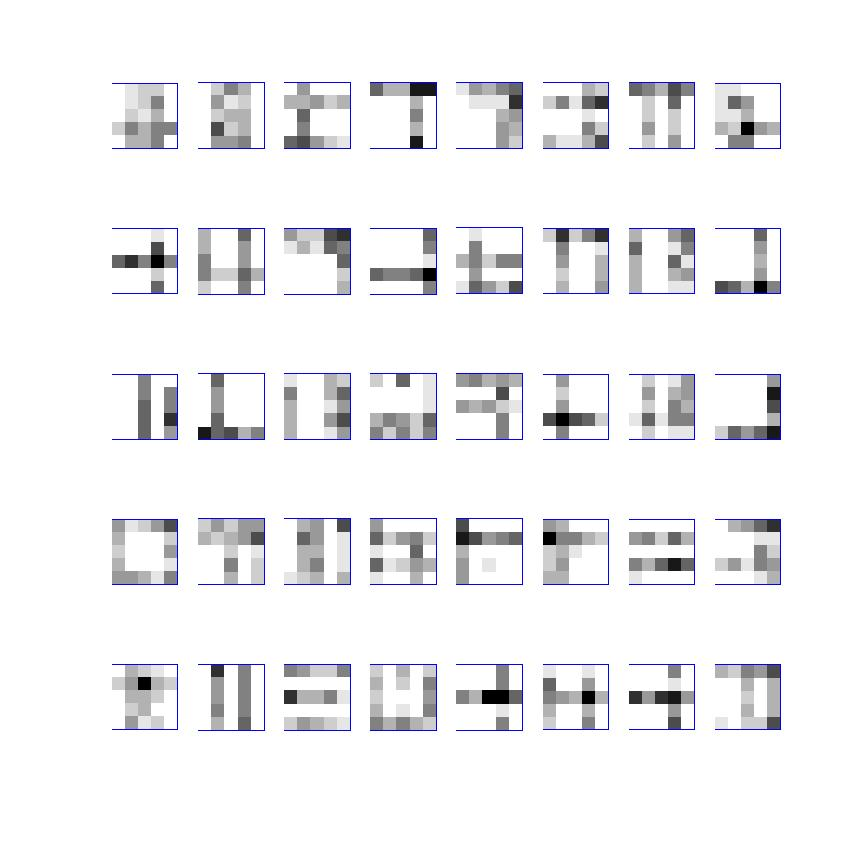
\includegraphics[width=3in,height=3in]{restau.jpg} 
    \caption{40 Restaurants}
\end{figure}

\subsection{ii) Initialization}
Run 5 times:
\begin{figure}[h] 
  \begin{minipage}[b]{0.5\textwidth} 
    \centering 
    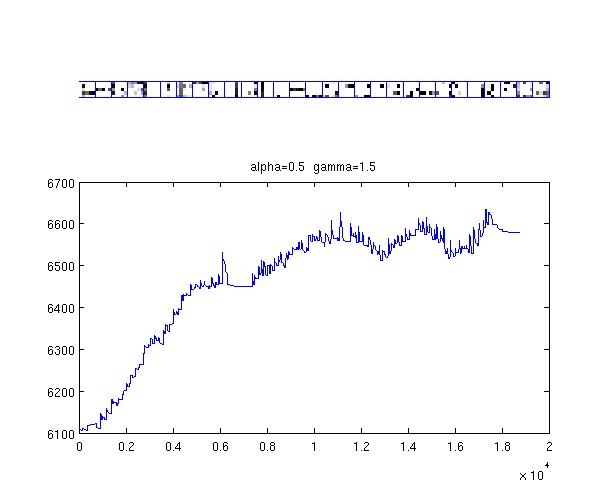
\includegraphics[width=3in,height=3in]{init1_5.jpg} 
    \caption{5 runs:Dish Config and -log Probability}
    \label{fig:by:table} 
  \end{minipage}% 
  \begin{minipage}[b]{0.5\textwidth} 
    \centering 
    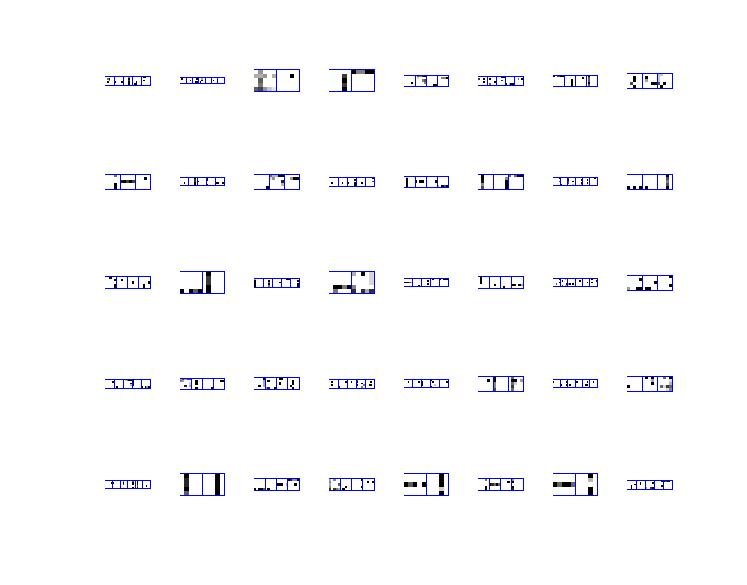
\includegraphics[width=3in,height=3in]{init1_5d.jpg} 
    \caption{5 runs:Table Config for 40 restaurants}
    \label{fig:by:table}  
   \end{minipage}% 
\end{figure}

\subsection{iii) Search}
1)run 40 times,search table during Split-Dish\\
\begin{figure}[h] 
  \begin{minipage}[b]{0.5\textwidth} 
    \centering 
    \includegraphics[width=3in,height=3in]{init1_5_mt5.jpg} 
    \caption{40 runs(merge table):Dish Config and -log Probability}
    \label{fig:by:table} 
  \end{minipage}% 
  \begin{minipage}[b]{0.5\textwidth} 
    \centering 
    \includegraphics[width=3in,height=3in]{init1_5_mt5d.jpg} 
    \caption{40 runs(merge table):Table Config for 40 restaurants}
    \label{fig:by:table}  
   \end{minipage}% 
\end{figure}
2)run 40 times,without searching table during Split-Dish\\
\begin{figure}[h] 
  \begin{minipage}[b]{0.5\textwidth} 
    \centering 
    \includegraphics[width=3in,height=3in]{init1_5_nmt.jpg} 
    \caption{40 runs(no merge table):Dish Config and -log Probability}
    \label{fig:by:table} 
  \end{minipage}% 
  \begin{minipage}[b]{0.5\textwidth} 
    \centering 
    \includegraphics[width=3in,height=3in]{init1_5_nmt5d.jpg} 
    \caption{40 runs(no merge table):Table Config for 40 restaurants}
    \label{fig:by:table}  
   \end{minipage}% 
\end{figure}



\section{3) Search}
Maximize the log likelihood:\\
$P=-log p(x,z|\lambda)$\\ =\\
(t-term)$ \underline{log \frac{\Gamma(m..+\gamma)}{\Gamma(\gamma)}+\sum_{j=1}^{J} \{log \frac{\Gamma(n_{j..}+\alpha)}{\Gamma(\alpha)}-\sum_{t=1}^{m_{j.}}[log(\Gamma(n_{jt.})+log \alpha
]\}}$\\ \\
+(k-term)$ \sum_{k=1}^{K} [log(\frac{\Gamma(n_{..k}+W\phi_{0})}{\Gamma(W\phi_{0})})+log(\Pi_{w=1}^{W}\frac{\Gamma(\phi_{0})}{\Gamma(\phi_{0}+n_{..k}^{w})})
-\underline{log(\Gamma(m_{.k})-log \gamma]}$\\ W:number of unique words\\ 
$n_{..k}^{w}$number of occurence of word w in dish k \\ \\ \\ 



\end{spacing}
\end{document}

%%%%%%%%%%%%%%%%%%%%%%%%%%%%%%%%%%%%%%%%%%%%%%%%%%%%%%%%%%%%%
